\laborator{Моделирование процесса теплообмена}

\goal составить математические модели теплообменных аппаратов с различной структурой потоков.

\subsubsection{Теория}
Практически ни одно производство в химической технологии не обходится без процессов теплообмена, когда необходимо осуществлять процессы нагрева охлаждения, испарения или конденсации.
 Процесс теплообмена может рассматриваться индивидуально (в случае теплообменников), или в совокупности с процессами массопередачи и химическими реакциями.

В зависимости от организации подвода или отвода тепла структура потока теплоносителей может описываться различными моделями. В связи с тем, что модель идеального вытеснения имеет наибольшую движущую силу, в промышленности наибольшее распространение получили аппараты наиболее близкие к данной структуре потока: кожухотрубчатые, <<труба в трубе>>, пластинчатые и другие. На рисунке  \ref{fig:heat.scheme1} представлена схема потоков в прямоточном теплообменнике.

\begin{figure}[h]
	\begin{center}
		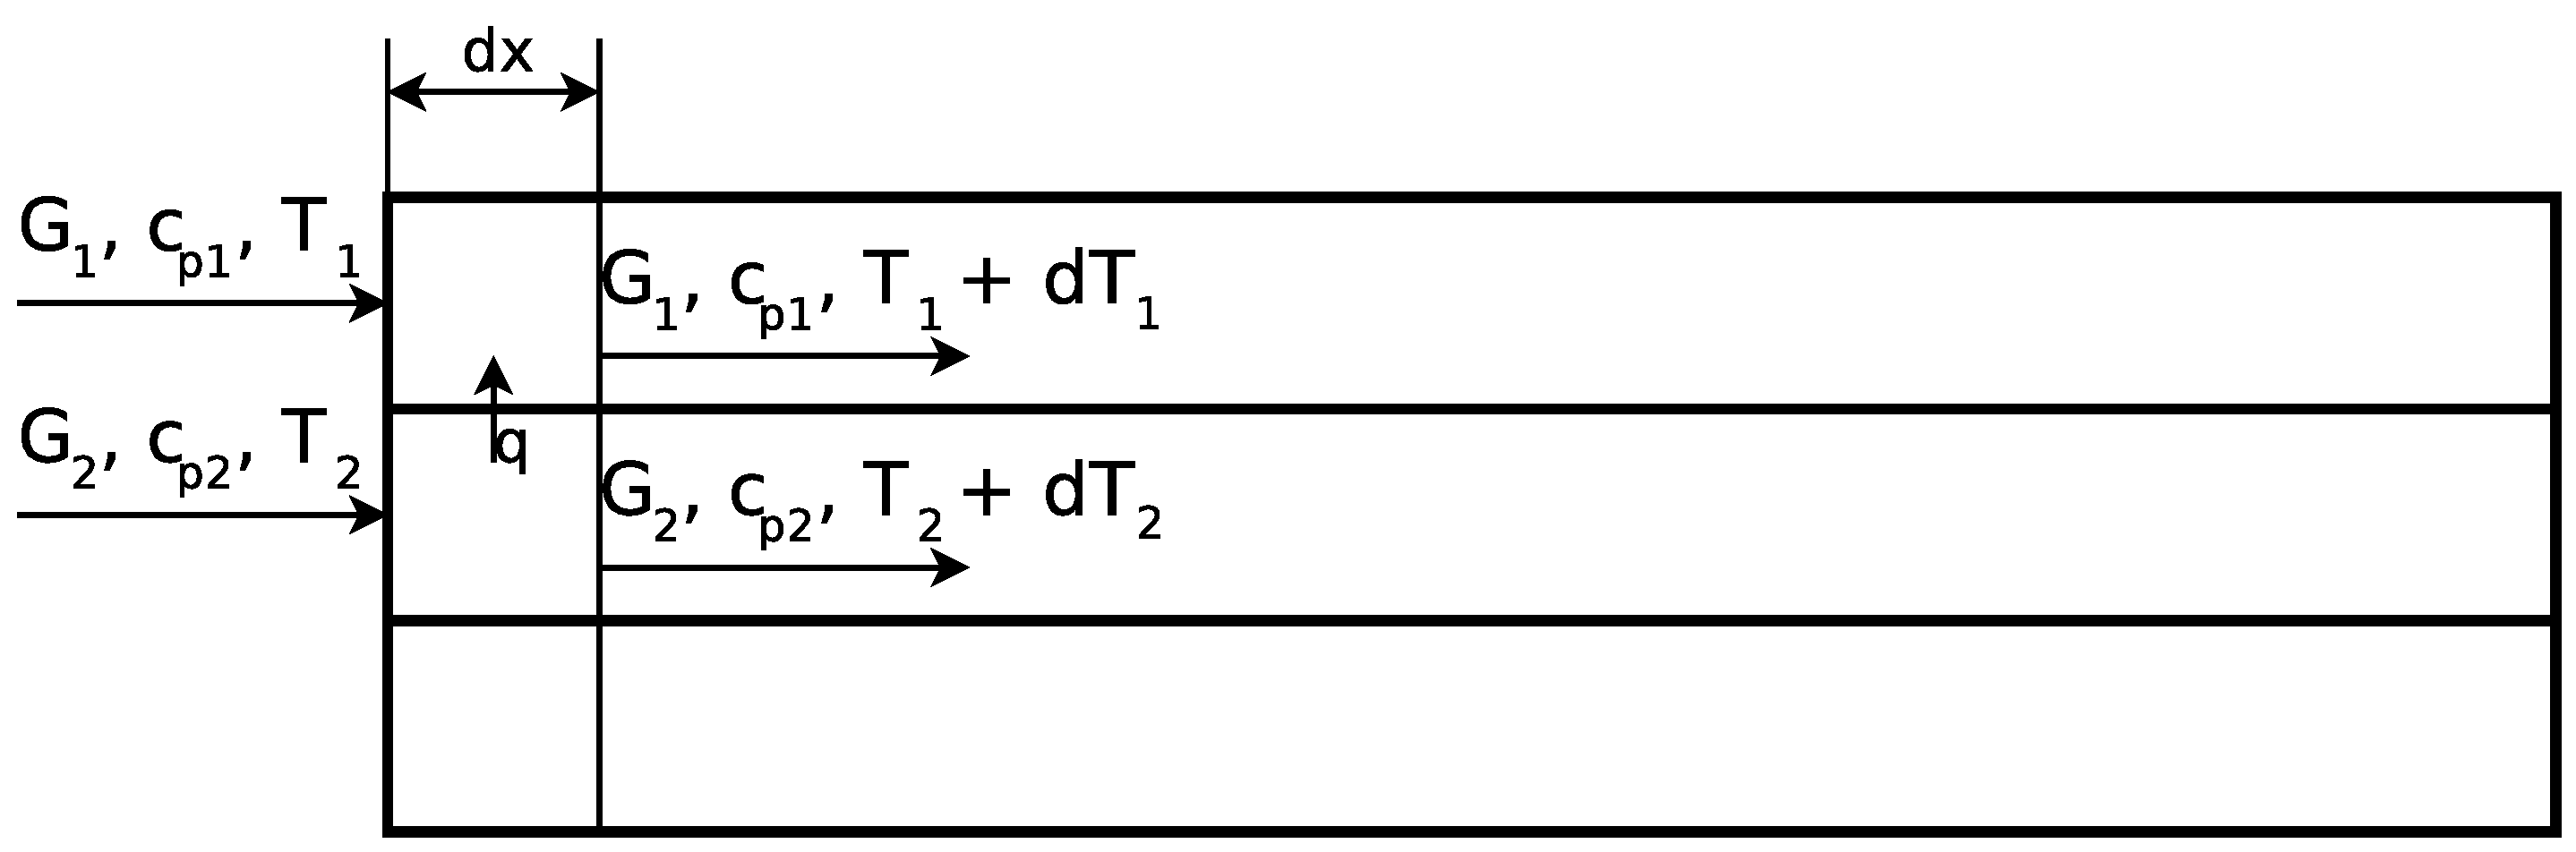
\includegraphics[width=\textwidth]{heat-scheme1.eps}
	\end{center}
	\caption{Схема потоков в прямоточном теплообменнике типа <<труба в трубе>>} \label{fig:heat.scheme1}
\end{figure}

\subsubsection*{Модель идеального вытеснения}
Для вывода уравнений модели идеального вытеснения запишем тепловой баланс холодного теплоносителя:
\begin{equation}\label{eq:tbal-cold}
	G_1 T_1 c_{p1}-G_1 c_{p1} (T_1+ d T_1) + q d F=0,
\end{equation}
где $G$ --- массовый расход теплоносителя, $c_p$ --- изобарная теплоемкость, $q$ --- тепловой поток, $F$ --- площадь поверхности теплообмена.

Поток тепла направлен от горячего теплоносителя к холодному, поэтому в выражении  теплового баланса горячего теплоносителя он будет с отрицательным знаком:
\begin{equation}\label{eq:tbal-hot}
	G_2 T_2 c_{p2} -G_2 c_{p2} (T_2 + d T_2) - q d F =0.
\end{equation}

Поток тепла можно выразить уравнением теплопередачи:
\begin{equation}\label{eq:teploper}
	q=K(T_2-T_1),
\end{equation}
где $K$ --- коэффициент теплопередачи. Расписывая площадь поверхности теплообмена через периметр сечения теплообмена $P$ и длину элементарного объема $d x$ как $d F = d x P$, с использованием выражения \eqref{eq:teploper}, уравнения \eqref{eq:tbal-cold} и \eqref{eq:tbal-hot} можно переписать в виде системы:

 \begin{equation} \label{eq:tep.pryamo}
 \left\{
 \begin{aligned}
 &\dfrac{dT_1}{dx}=\dfrac{K(T_2-T_1)P}{G_1 c_{p1}}        \\
 &\dfrac{dT_2}{dx}=-\dfrac{K(T_2-T_1)P}{G_2 c_{p2}}            
 \end{aligned}
 \right. .
 \end{equation}

В зависимости от поставленной задачи граничные условия могут задаваться по разному. Обычно известны расходы теплоносителей и температуры на входе теплообменника. Таким образом, в случае прямоточного теплообменника, для определения температур теплоносителя по длине теплообменника решается задача Коши. 

Для противоточного теплообменника изменяется направление движения одного из теплоносителей. Таким образом, переписывая выражения тепловых балансов,  можно записать следующую систему дифференциальных уравнений:
 \begin{equation}\label{eq:tep.protivo}
 \left\{
 \begin{aligned}
 &\dfrac{dT_1}{dx}=\dfrac{K(T_2-T_1)P}{G_1 c_{p1}}        \\
 &\dfrac{dT_2}{dx}=\dfrac{K(T_2-T_1)P}{G_2 c_{p2}}            
 \end{aligned}
 \right. .
 \end{equation}
 
В случае противоточного теплообменника и известных входящих потоках необходимо решать краевую задачу.

\subsubsection*{Модель идеального смешения}
Согласно модели идеального смешения элементы потока в аппарате попадая в аппарат моментально перемешиваются по всему объему. Выражение для модели идеального смешения можно получить из теплового баланса всего теплообменника:
\begin{equation}
G_1 T_{1н} c_{p1}-G_1 c_{p1} T_1 + q F=0,
\end{equation}
где $T_{1н}$ --- температура на входе в теплообменник.
Данное выражение аналогично записи теплового баланса для элементарного объема теплообменника \eqref{eq:tbal-cold}. Подставляя выражение для теплового потока \eqref{eq:teploper} и преобразуя получим:
\begin{equation}
T_1-T_{1н} = \dfrac{K(T_1-T_2)F}{G_1 c_{p1}}.
\end{equation}

\subsubsection*{Ячеечная модель}
Ячеечная представляет из себя несколько последовательно соединенных ячеек идеального смешения. Для каждой из ячеек можно записать тепловой баланс и получить систему алгебраических уравнений. Пример алгебраической системы, когда обогрев теплоносителя осуществляется конденсирующимся паром (температура второго теплоносителя постоянная и равная $T_{vap}$):
 \begin{equation}\label{eq:tep.yam}
\left\{
\begin{aligned}
&G c_p ( T_{1} - T_{in} ) = K_1 \dfrac {F} {m} ( T_{vap} - T_{1} )        \\
&G c_p ( T_{2} - T_{1} ) = K_2 \dfrac {F} {m} ( T_{vap} - T_{2} )	\\
& ... \\
&G c_p ( T_{m} - T_{m-1} ) = K_m \dfrac {F} {m} ( T_{vap} - T_{m} )           
\end{aligned}
\right. ,
\end{equation}
где $m$ --- количество ячеек, $T_{in}$ --- температура на входе в теплообменник.


Для решения описанных выше уравнений или систем уравнений необходимо вычислить значение коэффициента теплопередачи. Приведем последовательность расчета коэффициентов теплопередачи по критериальным уравнениям для теплообменника типа <<труба в трубе>>.

Определяется усредненная по сечению скорость теплоносителей:
\begin{equation}
	\bar{w} = \dfrac{ G}{\rho S},
\end{equation}
где $S$ --- площадь поперечного сечения потока жидкости, $\rho$ --- плотность теплоносителя.
Рассчитываются критерии:
Рейнольдса:
\begin{equation} \label{eq.tepl.re}
Re=\dfrac{\bar{w} l \rho}{\mu},
\end{equation}
Прандтля:
\begin{equation} \label{eq.tepl.pr}
Pr=\dfrac{\mu c_p}{\lambda},
\end{equation}
Грасгофа:
\begin{equation}
Gr= g l^3 \beta_p \rho^2 \dfrac{\Delta T}{\mu^2},
\end{equation}
где $l$ --- характерный геометрический размер аппарата, $\mu$ --- коэффициент динамической вязкости теплоносителя, $\lambda$ --- коэффициент теплопроводности теплоносителя, $\beta_p$ --- коэффициент объемного расширения теплоносителя, $\Delta T$ --- движущая сила теплоотдачи. При расчете коэффициента теплоотдачи в трубах в качестве характерного геометрического размера при определении критериев подобия выступает эквивалентный диаметр $D_э=\dfrac{4S}{P}$, где $S$ --- площадь сечения, $P$ --- полный периметр сечения потока, независимо от того, какая часть участвует в теплообмене.

Коэффициент теплоотдачи входит в выражение для критерия Нуссельта: 
\begin{equation} \label{eq.tepl.nu}
	Nu=\dfrac{\alpha l}{\lambda}.
\end{equation}
При определении коэффициента теплоотдачи критериальное уравнение представляют в виде функции:
\begin{equation}
	Nu= f (Re, Pr, Gr, ...),
\end{equation}
вид которой зависит от многих факторов: конструкции аппарата, скорости движения жидкости, фазового состояния теплоносителей, физико-химических свойств и т.д. 

Для прямых труб круглого сечения критерий Нуссельта зависит от режима течения \cite{posobie}. Для турбулентного режима, когда $Re>10000$ используется выражение:
\begin{equation} \label{eq:kt-1}
	Nu=0.021 Re^{0.8} Pr^{0.43} \left( \dfrac{Pr}{Pr_{гр}} \right) ^{0.25} .
\end{equation}
Для переходного и ламинарного режимов необходимо учитывать явление естественной конвекции, когда возникают дополнительные потоки за счет различной плотности вследствие неравномерного нагрева:

$Gr Pr < 8 \cdot 10^5$ и $Re < 2300 $:
\begin{equation} \label{eq:kt-2}
	Nu=1.55 \left(  Re Pr \dfrac{d_э}{2L}\right) ^ {1/3} \left( \dfrac{\mu}{\mu_{гр}} \right) ^{0.14},
\end{equation}
где $L$ --- длина теплообменника.

 $Gr Pr < 8 \cdot 10^5$ и $2300 <Re < 10000 $:
\begin{equation} \label{eq:kt-3}
	Nu=(-6.1 +4.75 \cdot 10^{-3} Re -8.14\cdot 10^{-8} Re^2) Pr^{0.43} \left( \dfrac{Pr}{Pr_{гр}} \right) ^{0.25}.
\end{equation}

$Gr Pr > 8 \cdot 10^5$ и $Re < 3500 $:
\begin{equation} \label{eq:kt-4}
Nu=0.8 \left( Re Pr \dfrac{d_э}{L}\right) ^{0.4} (Gr Pr)^{0.1} \left( \dfrac{\mu}{\mu_{гр}} \right) ^{0.14},
\end{equation}
если $Gr Pr > 8 \cdot 10^5$ и $3500 <Re < 10000 $:
\begin{equation} \label{eq:kt-5}
Nu=0.022 Re^{0.8} Pr^{0.4} \left( \dfrac{\mu}{\mu_{гр}} \right) ^{n},
\end{equation}
где $n = 0.11$ для холодного теплоносителя, $n = 0.25$ --- для горячего. При расчете критериев Рейнольдса \eqref{eq.tepl.re}  и Прантля \eqref{eq.tepl.pr} используются теплофизические свойства, которые зависят от температуры. Для выражений \eqref{eq:kt-1} и \eqref{eq:kt-3} свойства определяются при средней температуре потока $\bar{T} = \frac{T_н + T_к}{2}$, для выражений \eqref{eq:kt-2}, \eqref{eq:kt-4}, \eqref{eq:kt-5} --- при средней температуре между ядром потока и температурой стенки $\frac{\bar{T} + \bar{T_{гр}}}{2}$. В данной лабораторной работе, для упрощения задачи не будет учитываться влияние температуры на свойства, это означает, что свойства в ядре потока и на границе будут одинаковые ($Pr=Pr_{гр}$ и $\mu = \mu_{гр}$).

При расчете процесса теплоотдачи в кольцевом канале выражения для критерия Нуссельта будут отличаться \cite{dit_posobie}:

турбулентный режим:
\begin{equation}
Nu=0.023 Re^{0.8} Pr^{0.4} \left(\dfrac{D_{вн}}{d_{н}}\right)^{0.45},
\end{equation}
где $D_{вн}$, $d_н$ --- внутренний и наружный  диаметр кольцевого сечения;

переходный режим ($2300 < Re < 10000$):
\begin{equation}
	Nu=0.008 Re^{0.9} Pr^{0.43},
\end{equation}

ламинарный режим ($Re < 2300$):
\begin{equation}
Nu=0.15 (Re Pr)^{0.33} (Gr Pr)^{0.1} \left( \dfrac{Pr}{Pr_{гр}} \right) ^{0.25}.
\end{equation}

Коэффициент теплоотдачи определяем через критерий Нуссельта \eqref{eq.tepl.nu} по выражению:
\begin{equation}
\alpha = \dfrac{Nu \lambda}{d_э}.
\end{equation}


Искомый коэффициент теплопередачи через плоскую стенку определяется по выражению:
\begin{equation}
	K=\dfrac{1}{\dfrac{1}{\alpha_1} + \sum \dfrac{\delta}{\lambda} + \dfrac{1}{\alpha_2}},
\end{equation}
где $\delta$ --- толщина стенки, разделяющей теплоносители, $\lambda$ --- коэффициент теплопроводности материала стенки, суммирование $\frac{\delta}{\lambda}$ проводится в случае если стенка состоит из нескольких слоев различного материала. 




 
%Ниже приведены выражения критерия Нуссельта для различных видов теплообменников и режимов течения:
% \begin{itemize}
%	 \item Теплоотдача в круглых трубах при турбулентном режиме ():
%		 
%	 \item Теплоотдача в круглых трубах при переходном режиме ($2300<Re<10000$):
%		 \begin{equation}
%		 	Nu=0.008 Re^{0.9} Pr^{0.43}.
%		 \end{equation}
%	 \item Теплоотдача в круглых трубах при ламинарном режиме течения:
%		\begin{equation}
%			Nu=0.17 Re^{0.33} Pr^{0.43} Gr^{0.1} \left( \dfrac{Pr}{Pr_{гр}} \right).
%		\end{equation}
%	 \item  
%	 \item Теплоотдача при перемешивании жидкостей мешалками:
%	 \begin{equation}
%		Nu=C Re^m Pr^{0.33} \left(\dfrac{\mu}{\mu_{ст}}\right)^{0.14} \dfrac{\lambda}{D}
%	 \end{equation}
%	 где критерий Рейнольдса определяется как $Re=\frac{ \rho n d_m^2}{\mu}$, $D$ --- диаметр емкости, $n$ --- частота вращения мешалки, $\mu_{ст}$ --- динамический коэффициент вязкости жидкости при температуре стенки змеевика или рубашки, $\mu$ --- коэффициент вязкости при средней температуре жидкости, определяемой $(t_{ср.ж}+t_{ст})/2$. Для аппаратов с рубашками: $C=0.36$, $m=0.67$
%\end{itemize}


\subsubsection*{Вопросы для самоконтроля:}
\begin{enumerate}
	\item Записать выражение теплового баланса теплообменника типа <<труба в трубе>> при наличии тепловых потерь.
	\item Как рассчитывается коэффициент теплопередачи?
	\item Как определяется коэффициент теплоотдачи?
\end{enumerate}

%В предлагаемых задачах можно считать теплофизические свойства не зависящими от температуры, следовательно в первом приближении  $\frac{Pr}{Pr_{ст}}=\frac{\mu}{\mu_{ст}}=1$, $\Delta T$ принять равным 5 С


\subsubsection*{Пример задания}
\begin{enumerate}
\item Вычислить распределение температур теплоносителей в прямоточном теплообменнике типа <<труба в трубе>>. Для обоих потоков использовать модель идеального вытеснения. Параметры теплообменника: длина  13.5~м, внутренний диаметр внешней трубы 32.5~мм,  внутренний диаметр внутренней трубы 17.2~мм, толщина стенки $\delta_{w}$=     4~мм,  теплопроводность материала стенки $\lambda_{w}=  453~\frac{\text{Вт}}{\text{м} \cdot \text{К}}$.  Горячий теплоноситель (обозначен индексом <<h>>) направляется во внутреннюю трубу и	 имеет следующие параметры: температура $\text{T}_{h}= 262~^\circ\mathrm{C}$, теплоемкость	  $c_{p{h}}= 3251.2~\frac{\text{Дж}}{\text{кг} \cdot ^\circ\mathrm{C}}$, теплопроводность 		$\lambda_{h}= 0.446~\frac{\text{Вт}}{\text{м} \cdot ^\circ\mathrm{C}}$, плотность 		$\rho_{h}= 1392 \frac{\text{кг}}{\text{м}^3}$, коэффициент вязкости $\mu_{h}=4.767 \text{мПа} 		\cdot \text{с} $, коэффициент термического расширения $\beta_{h}=0.000737 ^\circ\mathrm{C}^{-1}$,		 расход $G_{h}= 2957.403 \frac{\text{кг}}{\text{ч}}$. Холодный теплоноситель (обозначен индексом <<c>>) 		 направляется в кольцевое сечение и имеет следующие параметры: температура $T_{c}=   25		 ~^\circ\mathrm{C}$, теплоемкость $c_{p{c}}= 2691 \frac{\text{Дж}}{\text{кг} \cdot ^\circ\mathrm{C}}$,			 теплопроводность $\lambda_{c}=0.150 \frac{\text{Вт}}{\text{м} \cdot ^\circ\mathrm{C}}$, плотность 			 $\rho_{c}=  1488~\frac{\text{кг}}{\text{м}^3}$, коэффициент вязкости $\mu_{c}=6.355~\text{мПа} \cdot \text{с} $, 			 расход $G_{c}=3211.48~\frac{\text{кг}}{\text{ч}}$. 

\item Определить распределение температуры теплоносителей вдоль поверхности теплообмена при изменении направления движения теплоносителей на противоточное. Коэффициент теплопередачи, свойства веществ и площадь теплообменника взять из первого задания.

\item Рассчитать распределение температуры теплоносителей вдоль поверхности теплообмена в теплообменнике, структура потоков в котором описывается ячеечной моделью. Количество ячеек для обоих теплоносителей $m = $ 3. Коэффициент теплопередачи, свойства веществ и площадь теплообменника взять из первого задания.

\item Определить площадь теплообмена для модели идеального смешения, необходимую для достижения температур на выходе из теплообменника таких же, как для модели идеального вытеснения (температуры взять из первого задания).
Для теплообменников с различной структурой потоков провести сравнение площади поверхности теплообмена, необходимой для достижения заданной температуры.
\end{enumerate}